\documentclass[6008notes.tex]{subfiles}
\begin{document}
\graphicspath{ {images/jointdist/} }

\section{Jointly Distributed Random Variables}

\subsection{Relating Two Random Variables}

At the most basic level, inference refers to using an observation to reason about some unknown quantity. In this course, the observation and the unknown quantity are represented by random variables. The main modeling question is: How do these random variables relate?

Let's build on our earlier weather example, where now another outcome of interest appears, the temperature, which we quantize into to possible values ``hot'' and ``cold''. Let's suppose that we have the following probability space:

{\centering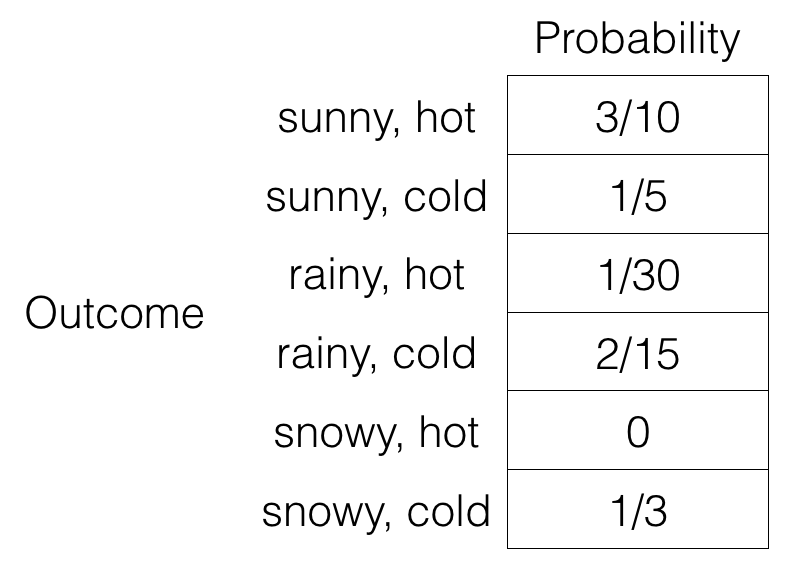
\includegraphics[scale=0.4]{images_sec-joint-rv-prob-space} \par}

You can check that the nonnegative entries do add to 1. If we let random variable $W$ be the weather (sunny, rainy, snowy) and random variable $T$ be the temperature (hot, cold), then notice that we could rearrange the table in the following fashion:

{\centering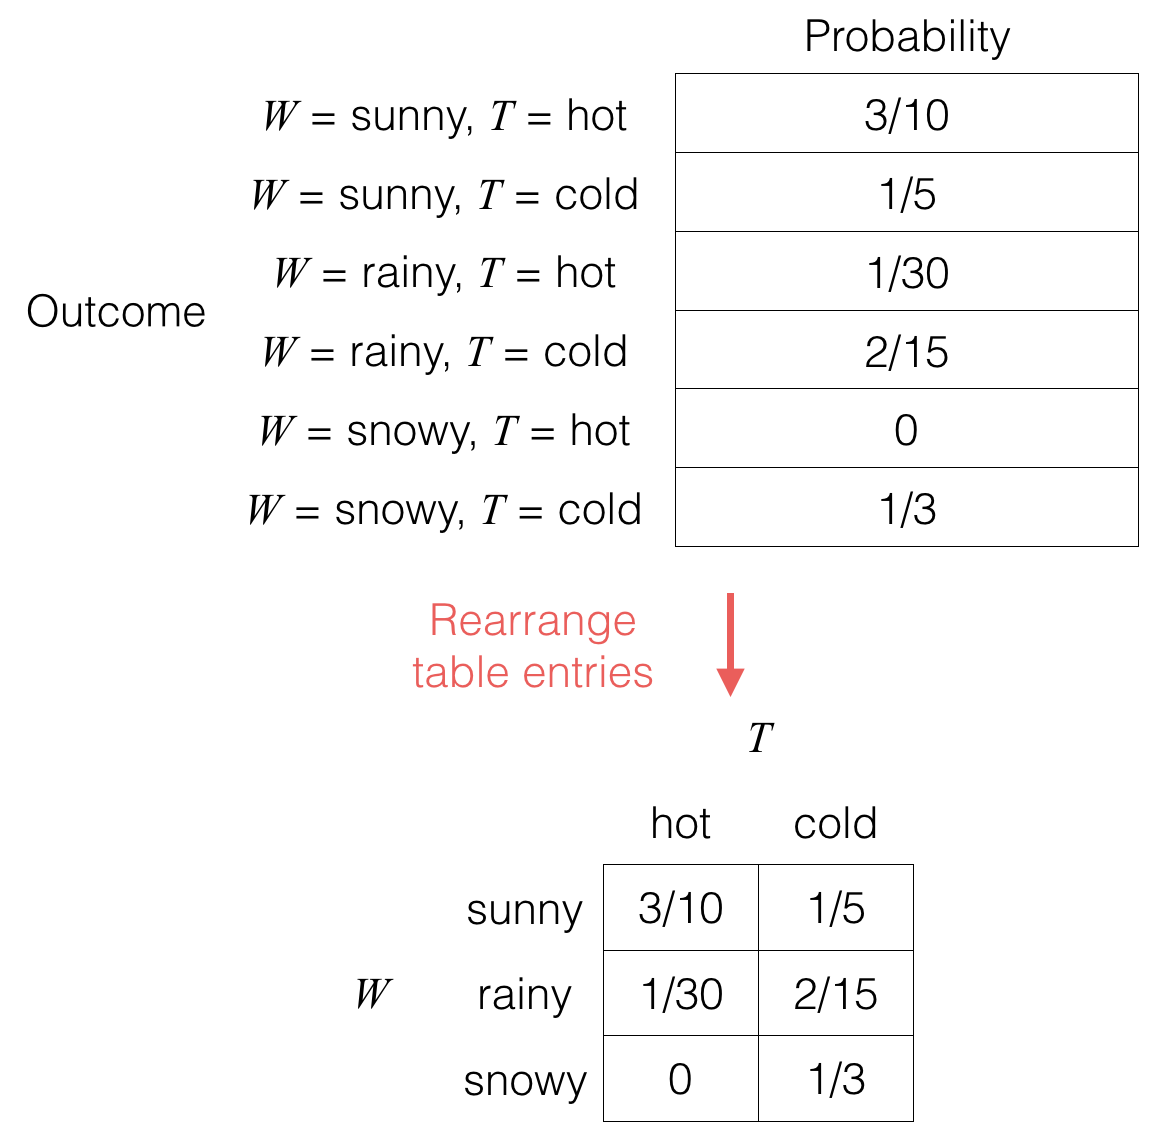
\includegraphics[scale=0.4]{images_sec-joint-rv-rearrange-table} \par}

When we talk about two separate random variables, we could view them either as a single ``super'' random variable that happens to consist of a pair of values (the first table; notice the label for each outcome corresponds to a pair of values), or we can view the two separate variables along their own different axes (the second table).

The first table tells us what the underlying probability space is, which includes what the sample space is (just read off the outcome names) and what the probability is for each of the possible outcomes for the underlying experiment at hand.

The second table is called a joint probability table $p_{W,T}$ for random variables $W$ and $T$, and we say that random variables $W$ and $T$ are jointly distributed with the above distribution. Since this table is a rearrangement of the earlier table, it also consists of nonnegative entries that add to 1.

The joint probability table gives probabilities in which $W$ and $T$ co-occur with specific values. For example, in the above, the event that ``$W=\text {sunny}$'' and the event that ``$T=\text {hot}$'' co-occur with probability 3/10. Notationally, we write

{\centering$p_{W,T}(\text {sunny},\text {hot})=\mathbb {P}(W=\text {sunny},T=\text {hot})=\frac{3}{10}.$ \par}
 
\paragraph{Conceptual note:} Given the joint probability table, we can easily go backwards and write out the first table above, which is the underlying probability space.

\paragraph{Preview of inference:} Inference is all about answering questions like ``if we observe that the weather is rainy, what is the probability that the temperature is cold?'' Let's take a look at how one might answer this question.

First, if we observe that it is rainy, then we know that ``sunny'' and ``snowy'' didn't happen so those rows aren't relevant anymore. So the space of possible realizations of the world has shrunk to two options now: $(W=\text {rainy},T=\text {hot})$ or $(W=\text {rainy},T=\text {cold})$. But what about the probabilities of these two realizations? It's not just 1/30 and 2/15 since these don't sum to 1 --- by observing things, adjustments can be made to the probabilities of different realizations but they should still form a valid probability space.

Why not just scale both 1/30 and 2/15 by the same constant so that they sum to 1? This can be done by dividing 1/30 and 2/15 by their sum:

{\centering$\text {hot:}\quad \frac{\frac{1}{30}}{\frac{1}{30}+\frac{2}{15}}=\frac{1}{5},\qquad 
 \text {cold}:\quad \frac{\frac{2}{15}}{\frac{1}{30}+\frac{2}{15}}=\frac{4}{5}.$ \par}
 
Now they sum to 1. It turns out that, given that we've observed the weather to be rainy, these are the correct probabilities for the two options ``hot'' and ``cold''. Let's formalize the steps. We work backwards, first explaining what the the denominator ``$\frac{1}{30}+\frac{2}{15}=\frac{1}{6}$'' above comes from.

\subsection{Representing a Joint Probability Table in Code}

There are various ways to represent a joint probability table in code. Here are a few.

Note that we have updated \href{https://d37djvu3ytnwxt.cloudfront.net/assets/courseware/v1/710ba23b569da54c14fc614315ced6a1/asset-v1:MITx+6.008.1x+3T2016+type@asset+block/comp_prob_inference.py}{\texttt{comp\_prob\_inference.py}}! Please re-download it!

\paragraph{Approach 0:} Don't actually represent the joint probability table. This doesn't store the 2D table at all but is a first attempt at coding up something that has all the information in the joint probability table. Specifically, we can just code up the entries like how we coded up a probability space:

\begin{lstlisting}
> prob_table = {('sunny', 'hot'): 3/10,
>     ('sunny', 'cold'): 1/5,
>     ('rainy', 'hot'): 1/30,
>     ('rainy', 'cold'): 2/15,
>     ('snowy', 'hot'): 0,
>     ('snowy', 'cold'): 1/3}
\end{lstlisting}

Thus, if we want the probability of $W=\text {rainy}$ and $T=\text {cold}$, we write:

\begin{lstlisting}
> prob_table[('rainy', 'cold')]
0.13333333333333333
\end{lstlisting}

Some times, this representation is sufficient. Given a specific weather and temperature stored as strings in \texttt{w} and \texttt{t} respectively, \lstinline{prob_table[(w, t)]} gives you the joint probability table evaluated at $W = \texttt{w}$ and $T = \texttt{t}$.

\paragraph{Approach 1:} Use dictionaries within a dictionary. This works as follows:

\begin{lstlisting}
> prob_W_T_dict = {}
> for w in {'sunny', 'rainy', 'snowy'}:
>     prob_W_T_dict[w] = {}
>
> prob_W_T_dict['sunny']['hot'] = 3/10
> prob_W_T_dict['sunny']['cold'] = 1/5
> prob_W_T_dict['rainy']['hot'] = 1/30
> prob_W_T_dict['rainy']['cold'] = 2/15
> prob_W_T_dict['snowy']['hot'] = 0
> prob_W_T_dict['snowy']['cold'] = 1/3
>
> comp_prob_inference.print_joint_prob_table_dict(prob_W_T_dict)
           cold       hot
rainy  0.133333  0.033333
snowy  0.333333  0.000000
sunny  0.200000  0.300000
\end{lstlisting}

Note that because dictionary keys aren't ordered, the row ordering and column ordering need not match the tables we have been showing in the course notes earlier. This is not a problem.

If we want the probability of $W=\text {rainy}$ and $T=\text {cold}$, we write:

\begin{lstlisting}
> prob_W_T_dict['rainy']['cold']
0.13333333333333333
\end{lstlisting}

The probability for $W =$ \texttt{w} and $T =$ \texttt{t} is stored in \lstinline{prob_W_T_dict[w][t]}.

\paragraph{Approach 2:} Use a 2D array. Another approach is to directly store the joint probability table as a 2D array, separately keeping track of what the rows and columns are. We use a NumPy array (but really you could use Python lists within a Python list, much like how the previous approach used dictionaries within a dictionary; the indexing syntax changes only slightly):

\begin{lstlisting}
> import numpy as np
> prob_W_T_rows = ['sunny', 'rainy', 'snowy']
> prob_W_T_cols = ['hot', 'cold']
> prob_W_T_array = np.array([[3/10, 1/5], [1/30, 2/15], [0, 1/3]])
> comp_prob_inference.print_joint_prob_table_array(prob_W_T_array, prob_W_T_rows, prob_W_T_cols)
            hot      cold
sunny  0.300000  0.200000
rainy  0.033333  0.133333
snowy  0.000000  0.333333
\end{lstlisting}

Note that the ordering of rows is specified, as is the ordering of the columns, unlike in the dictionaries within a dictionary representation.

Retrieving a specific table entry requires a little bit more code since we need to figure out what the row and column numbers are corresponding to a specific pair of row and column labels. For example, if we want the probability of $W=\text {rainy}$ and $T=\text {cold}$, we write:

\begin{lstlisting}
> prob_W_T_array[prob_W_T_rows.index('rainy'), prob_W_T_cols.index('cold')]
0.13333333333333333
\end{lstlisting}

Note that \texttt{prob\_W\_T\_rows.index('rainy')} finds the row number (starting from 0) corresponding to ``rainy''.

Using \texttt{.index} does a search through the whole list of row/column labels, which for large lists can be slow. Let's fix this!

A cleaner and faster way is to create separate dictionaries mapping the row and column labels to row and column indices in the 2D array. In other words, instead of writing \lstinline{prob_W_T_rows.index('rainy')} to find the row number for 'rainy', we want to just be able to write something like \lstinline{prob_W_T_row_mapping['rainy']}, which returns the row number. We can define Python variable \lstinline{prob_W_T_row_mapping} as follows:

\begin{lstlisting}
> prob_W_T_row_mapping = {}
> for index, label in enumerate(prob_W_T_rows):
>     prob_W_T_row_mapping[label] = index
\end{lstlisting}

Note that \lstinline{enumerate(prob_W_T_rows)} produces an iterator that consists of pairs \lstinline{(0, 'sunny'), (1, 'rainy'), (2, 'snowy')}. You can see this by entering:

\begin{lstlisting}
> print(list(enumerate(prob_W_T_rows)))
[(0, 'sunny'), (1, 'rainy'), (2, 'snowy')]
\end{lstlisting}

Note that each pair consists of the row number followed by the label.

In fact, the three lines we used to define \lstinline{prob_W_T_row_mapping} can be written in one line with a Python dictionary comprehension:

\begin{lstlisting}
> prob_W_T_row_mapping = {label: index for index, label in enumerate(prob_W_T_rows)}
\end{lstlisting}

We can do the same thing to define a mapping of column labels to column numbers:

\begin{lstlisting}
> prob_W_T_col_mapping = {label: index for index, label in enumerate(prob_W_T_cols)}
\end{lstlisting}

In summary, we can represent the joint probability table as follows:

\begin{lstlisting}
> prob_W_T_rows = ['sunny', 'rainy', 'snowy']
> prob_W_T_cols = ['hot', 'cold']
> prob_W_T_row_mapping = {label: index for index, label in enumerate(prob_W_T_rows)}
> prob_W_T_col_mapping = {label: index for index, label in enumerate(prob_W_T_cols)}
> prob_W_T_array = np.array([[3/10, 1/5], [1/30, 2/15], [0, 1/3]])
\end{lstlisting}

Now the probability for $W =$ \texttt{w} and $T =$ \texttt{t} is given by:

\begin{lstlisting}
> prob_W_T_array[prob_W_T_row_mapping[w], prob_W_T_col_mapping[t]]
\end{lstlisting}

\paragraph{Some remarks:} The 2D array representation, as we'll see soon, is very easy to work with when it comes to basic operations like summing rows, and retrieving a specific row or column. The main disadvantage of this representation is that you need to store the whole array, and if the alphabet sizes of the random variables are very large, then storing the array will take a lot of space!

The dictionaries within a dictionary representation allows for easily retrieving rows but not columns (try it: write a Python function that picks out a specific row and another function that picks out a specific column; you should see that retrieving a row is easier because it corresponds to looking at the value stored for a single key of the outer dictionary). This also means that summing a column's probabilities is more cumbersome than summing a row's probabilities. However, a huge advantage of this way of representing a joint probability table is that in many problems, we have a massive joint probability table that is mostly filled with 0's. Thus, the 2D array representation would require storing a very, very large table with many 0's, whereas the dictionaries within a dictionary representation is able to only store the nonzero table entries. We'll see more about this issue when we look at robot localization in the second section of the course on inference in graphical models.

\subsection{Marginalization}

Given a joint probability table, often we'll want to know what the probability table is for just one of the random variables. We can do this by just summing or ``marginalizing'' out the other random variables. For example, to get the probability table for random variable $W$, we do the following:

{\centering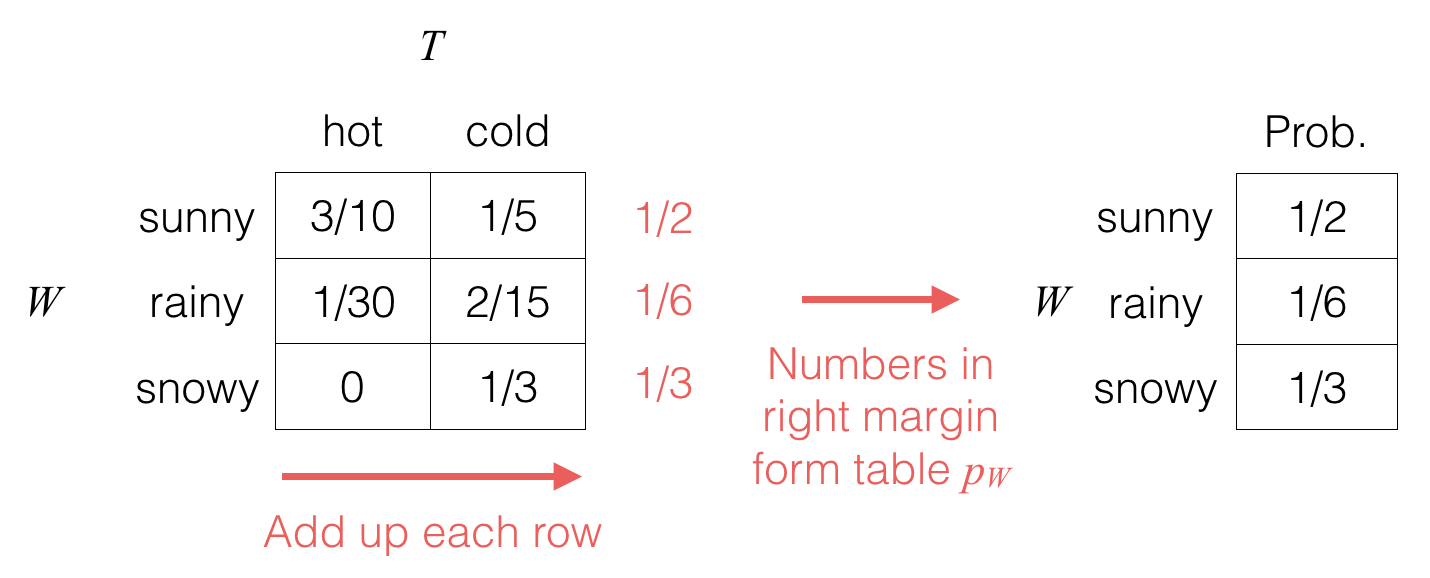
\includegraphics[scale=0.4]{images_sec-joint-rv-marg-rows} \par}

We take the joint probability table (left-hand side) and compute out the row sums (which we've written in the margin).

The right-hand side table is the probability table $p_W$ for random variable $W$; we call this resulting probability distribution the marginal distribution of $W$ (put another way, it is the distribution obtained by marginalizing out the random variables that aren't $W$).

In terms of notation, the above marginalization procedure whereby we used the joint distribution of $W$ and $T$ to produce the marginal distribution of $W$ is written:

{\centering$p_{W}(w)=\sum _{t\in \mathcal{T}}p_{W,T}(w,t),$ \par}
 
where $\mathcal{T}$ is the set of values that random variable $T$ can take on. In fact, throughout this course, we will often omit explicitly writing out the alphabet of values that a random variable takes on, e.g., writing instead

{\centering$p_{W}(w)=\sum _{t}p_{W,T}(w,t).$ \par}
 
It's clear from context that we're summing over all possible values for $t$, which is going to be the values that random variable $T$ can possibly take on.

As a specific example,

{\centering$p_{W}(\text {rainy})=\sum _{t}p_{W,T}(\text {rainy},t)=\underbrace{p_{W,T}(\text {rainy},\text {hot})}_{1/30}+\underbrace{p_{W,T}(\text {rainy},\text {cold})}_{2/15}=\frac{1}{6}.$ \par}
 
We could similarly marginalize out random variable $W$ to get the marginal distribution $p_T$ for random variable $T$:

{\centering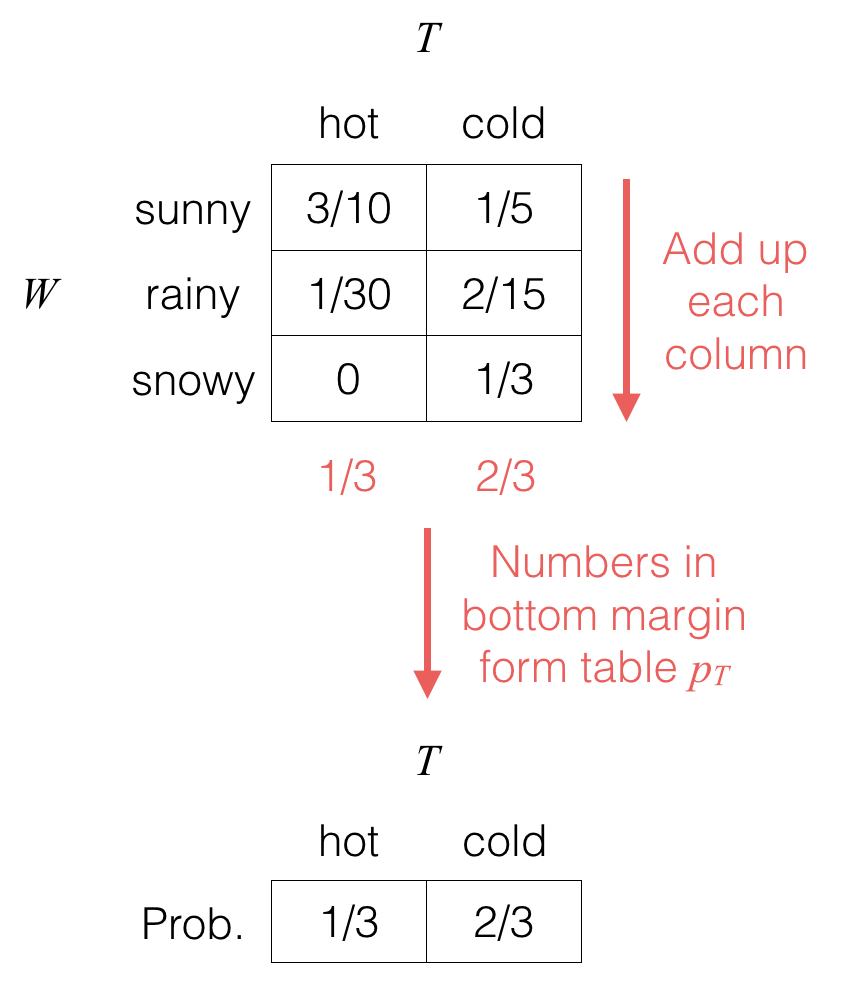
\includegraphics[scale=0.4]{images_sec-joint-rv-marg-cols} \par}

(Note that whether we write a probability table for a single variable horizontally or vertically doesn't actually matter.)

As a formula, we would write:

{\centering$p_{T}(t)=\sum _{w}p_{W,T}(w,t).$ \par}
 
For example,

{\centering$p_{T}(\text {hot})=\sum _{w}p_{W,T}(w,\text {hot})=\underbrace{p_{W,T}(\text {sunny},\text {hot})}_{3/10}+\underbrace{p_{W,T}(\text {rainy},\text {hot})}_{1/30}+\underbrace{p_{W,T}(\text {snowy},\text {hot})}_{0}=\frac{1}{3}.$ \par}
 
In general:

\paragraph{Marginalization:} Consider two random variables $X$ and $Y$ (that take on values in the sets $\mathcal{X}$ and $\mathcal{Y}$ respectively) with joint probability table $p_{X,Y}$. For any $x\in \mathcal{X}$, the marginal probability that $X=x$ is given by

{\centering$p_{X}(x)=\sum _{y}p_{X,Y}(x,y).$ \par}
 
\subsection{Marginalization for Many Random Variables}

What happens when we have more than two random variables? Let's build on our earlier example and suppose that in addition to weather $W$ and temperature $T$, we also had a random variable $H$ for humidity that takes on values in the alphabet {dry, humid}. Then having a third random variable, we can draw out a 3D joint probability table for random variables $W$, $T$, and $H$. As an example, we could have the following:

{\centering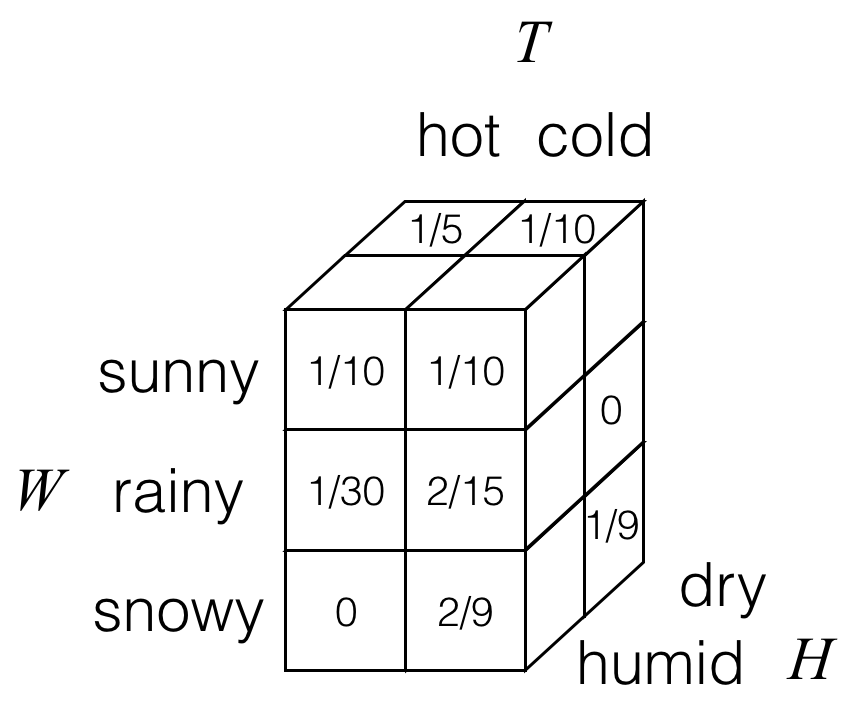
\includegraphics[scale=0.4]{images_sec-joint-rv-marg-many-rv-joint-table} \par}

Here, each of the cubes/boxes stores a probability. Not visible are two of the cubes in the back left column, which for this particular example both have probability values of 0.

Then to marginalize out the humidity $H$, we would add values as follows:

{\centering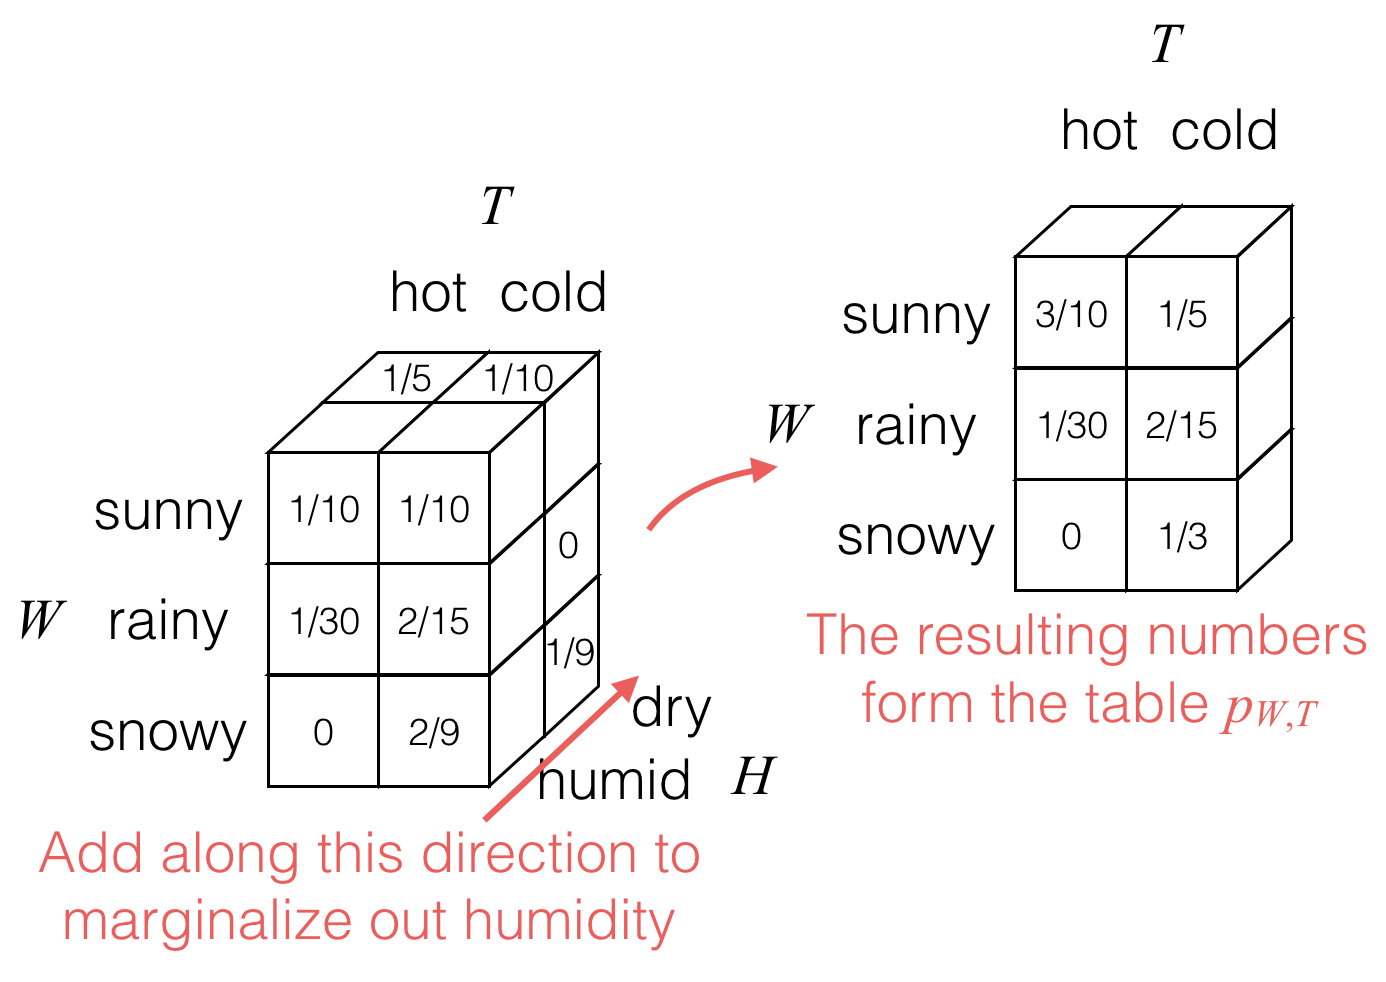
\includegraphics[scale=0.45]{images_sec-joint-rv-marg-many-rv-marg} \par}

The result is the joint probability table for weather $W$ and temperature $T$, shown still in 3D cubes with each cube storing a single probability.

As an equation:

{\centering$p_{W,T}(w,t) = \sum _ h p_{W,T,H}(w, t, h).$ \par}
 
In general, for three random variables X, Y, and Z with joint probability table pX,Y,Z, we have

\begin{eqnarray*}
p_{X,Y}(x,y)
&=&
\sum_{z} p_{X,Y,Z}(x,y,z), \\
p_{X,Z}(x,z)
&=&
\sum_{y} p_{X,Y,Z}(x,y,z), \\
p_{Y,Z}(y,z)
&=&
\sum_{x} p_{X,Y,Z}(x,y,z).
\end{eqnarray*}

Note that we can marginalize out different random variables in succession. For example, given joint probability table $p_{X,Y,Z}$, if we wanted the probability table $p_X$, we can get it by marginalizing out the two random variables $Y$ and $Z$:

{\centering$p_ X(x) = \sum _{y} p_{X,Y}(x,y) = \sum _{y} \Big( \sum _{z} p_{X,Y,Z}(x,y,z) \Big).$ \par}
 
Even with more than three random variables, the idea is the same. For example, with four random variables $W$, $X$, $Y$, and $Z$ with joint probability table $p_{W,X,Y,Z}$, if we want the joint probability table for $X$ and $Y$, we would do the following:

{\centering$p_{X,Y}(x, y) = \sum _ w \Big( \sum _ z p_{W,X,Y,Z}(w,x,y,z) \Big).$ \par}
 
\subsection{Conditioning for Random Variables}

When we observe that a random variable takes on a specific value (such as $W=\text {rainy}$ from earlier for which we say that we condition on random variable $W$ taking on the value ``rainy''), this observation can affect what we think are likely or unlikely values for another random variable.

When we condition on $W=\text {rainy}$, we do a two-step procedure; first, we only keep the row for $W$ corresponding to the observed value:

{\centering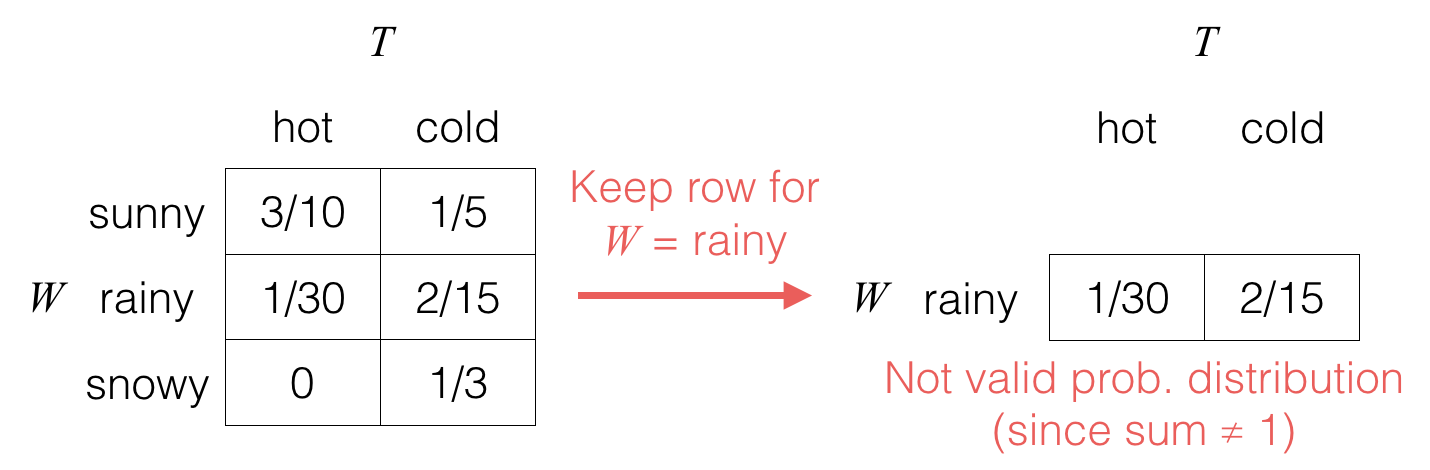
\includegraphics[scale=0.4]{images_sec-joint-rv-cond-restrict} \par}

Second, we ``normalize'' the table so that its entries add up to 1, which corresponds to dividing it by the sum of the entries, which is equal to $p_{W}(\text {rainy})$ in this case:

{\centering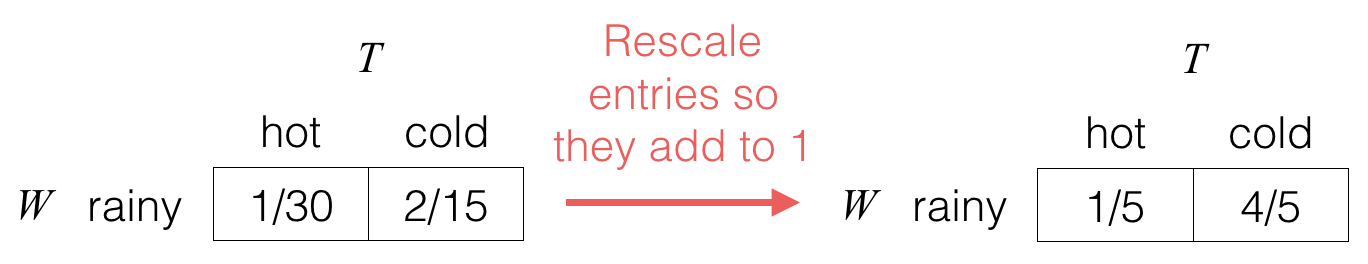
\includegraphics[scale=0.4]{images_sec-joint-rv-cond-renormalize} \par}

Notation: The resulting probability table $p_{T\mid W}(\cdot \mid \text {rainy})$ is associated with the random variable denoted $(T\mid W=\text {rainy})$; we use ``|'' to denote that we're conditioning on things to the right of ``|'' happening (these are things that we have observed or that we are given as having happened). We read ``$T\mid W=\text {rainy}$'' as either ``$T$ given $W$ is rainy'' or ``$T$ conditioned on $W$ being rainy''. To refer to specific entries of the table, we write, for instance,

{\centering$p_{T\mid W}(\text {cold}\mid \text {rainy})=\mathbb {P}(T=\text {cold}\mid W=\text {rainy})=\frac{4}{5}.$ \par}
 
In general:

\paragraph{Conditioning:} Consider two random variables $X$ and $Y$ (that take on values in the sets $\mathcal{X}$ and $\mathcal{Y}$ respectively) with joint probability table $p_{X,Y}$ (from which by marginalization we can readily compute the marginal probability table $p_Y$). For any $x\in \mathcal{X}$ and $y\in \mathcal{Y}$ such that $p_{Y}(y)>0$, the conditional probability of event $X=x$ given event $Y=y$ has happened is

{\centering$p_{X\mid Y}(x\mid y)\triangleq \frac{p_{X,Y}(x,y)}{p_{Y}(y)}.$ \par}
 
For example,

{\centering$p_{T\mid W}(\text {cold}\mid \text {rainy})=\frac{p_{W,T}(\text {rainy},\text {cold})}{p_{W}(\text {rainy})}=\frac{\frac{2}{15}}{\frac{1}{6}}=\frac{4}{5}.$ \par}
 
\paragraph{Computational interpretation:} To compute $p_{X\mid Y}(x\mid y)$, take the entry $p_{X,Y}(x,y)$ in the joint probability table corresponding to $X=x$ and $Y=y$, and then divide the entry by $p_Y(y)$, which is an entry in the marginal probability table $p_Y$ for random variable $Y$.

\subsection{Moving Toward a More General Story for Conditioning}

Jointly distributed random variables play a central role in this course. Remember that we will model observations as random variables and the quantities we want to infer also as random variables. When these random variables are jointly distributed so that we have a probabilistic way to describe how they relate (through their joint probability table), then we can systematically and quantitatively produce inferences.

We just saw how to condition on a random variable taking on a specific value. What about if we wanted to condition on a random variable taking on any one of of many values rather just one specific value? To answer this question, we look at a more general story of conditioning which is in terms of events.



\end{document}